\section{Background}

Dynamic memory allocation is an essential activity in most of the applications. It happens when an application needs a piece of memory whose size cannot be determined until runtime. Most systems support some system calls that could dynamically assign some memory to an application. When an application asks for some dynamic memory from the operating system, the simplest way is to give the exact size of memory it requests through these system calls, and to retrieve that memory back as soon as the application frees it. However, these allocation and deallocation system calls are usually much slower than other operations. So frequently allocating memory directly from the system is impractical for most of the applications. 

Memory allocators have risen to solve this problem using different allocation strategies. Usually applications communicate with the operating system in terms of memory only through their memory allocators. The idea of these allocators is trying to hold and manage some extra memory applied from the system and use them to serve latter memory request from the application as effiecently as possible. On the other hand, when a piece of memory is freed by the application, before released to the system it is handled by memory allocators in case there is a memory request in the same size in the near future. So it works like a memory buffer between an application and the system. Different ways of memory management significantly influence the performance of an application in terms of both memory and time.

\subsection{Dlmalloc}

Many memory allocation strategies and managers have been proposed and studied by many researchers. Among them, Doug Lea's malloc (\emph{dlmalloc}) \cite{lea1996memory} is ``among the fastest, most space-conserving, tunable, and portable general purpose allocators''. A study of Berger et al\cite{Berger:2002:RCM:583854.582421} shows that many other custom memory allocators don't perform significantly better than \emph{dlmalloc}, sometimes even worse. So in this paper, we choose \emph{dlmalloc} as our starting point and optimize its configuration to each of the subject applications.

\begin{figure}[htbp]
\centering
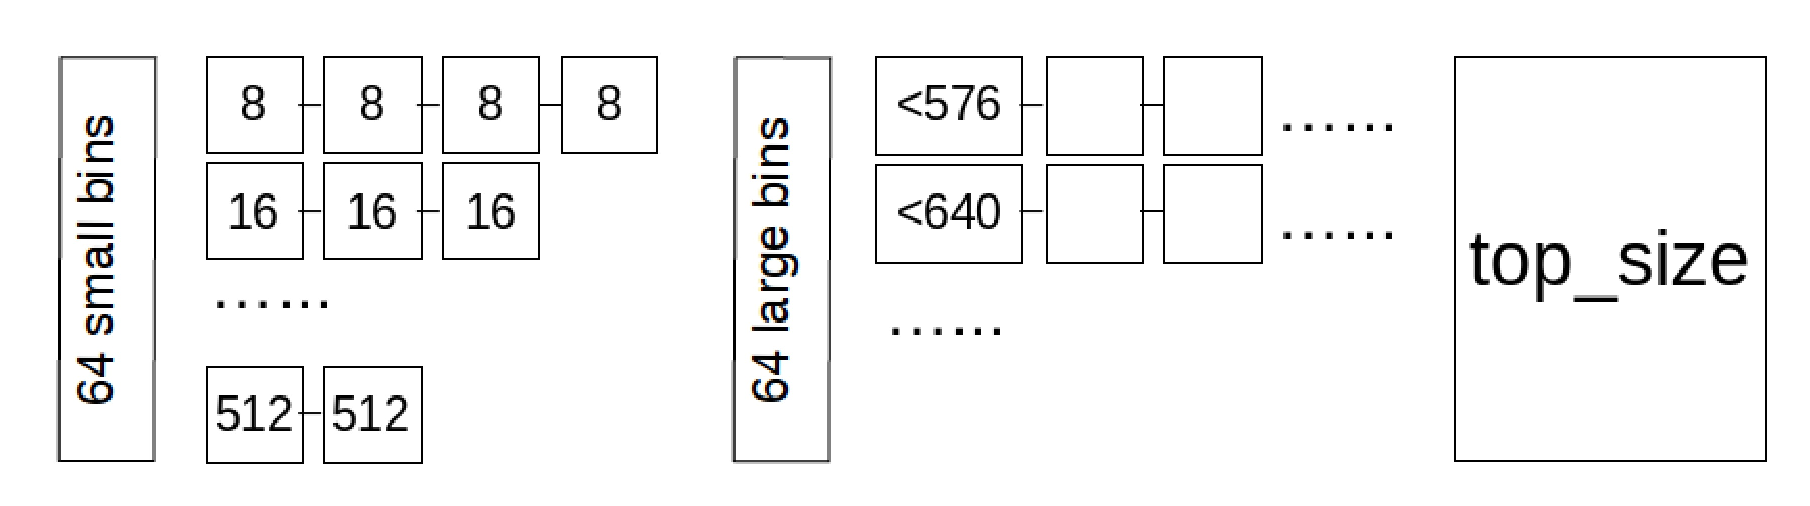
\includegraphics[width=3.2in]{fig7}
\caption{structure of \emph{dlmalloc}}\label{fig_7}
\end{figure}

\emph{Dlmalloc} is a general purpose memory allocator designed for c programs. It keeps two set of segregated lists managing small and large size available chunks respectively. Each of the segregated lists is called a bin and there are 64 small bins and 64 large bins in \emph{dlmalloc} (Figure \ref{fig_7}). For small bins, each one contains chunks in the exact same size, in which way insertion to or deletion from the list is very quick. For large bins, each bin is associated with a range of sizes and any free chunks within that range are stored in the corresponding bin in the ascending order. So managing large bins is more costly than small bins but fortunately large bins are less frequent than small bins. Apart from these bins, \emph{dlmalloc} also keeps a top chunk, which is always at the end of the heap so that it can be extended or trimmed without affecting other memory chunks. 

The top chunk is used only when there is no available chunk in any bins that meets the memory request. If the request size is too large to be satisfied from the top chunk and bigger than a pre-defined threshold, \emph{dlmalloc} uses an \emph{mmap}-like system call to allocate this size of memory from the operating system directly. Or it tries to extend the top chunk using \emph{sbrk}-like system call, so that the extended top chunk is big enough to cover the request.
When a chunk is freed by the application, it is put back to one of the bins according to its size, after which \emph{dlmalloc} occasionally coalesces contiguous free chunks to create bigger chunks. If the top chunk is enlarged by combining free chunks next to it, it could be trimmed if it is too large for the need of the application if the freed chunk was mapped directly from the system, it is released to the system immediately. 

% Intruduce the 9 parameters defined in Dlmalloc (1 paragraph)
% draw a table with "para name, type, range, default, comment"
\begin{table*}[htbp]
\centering
\caption{Selective \emph{dlmalloc} parameters}
\label{tab_dlmalloc_parameters}
\resizebox{0.9\textwidth}{!}{
\begin{tabular}{c|c|c|c|c}
\hline
Name & Default & Range & Type & Description\\
\hline
MALLOC\_ALIGNMENT & $2*sizeof(void*)$ & $(1~16)*sizeof(void*)$ & $2^n*sizeof(void*)$ & Alignment unit\\
\hline
FOOTERS & \emph{false} & \emph{true} or \emph{false} & boolean & Additional information of each chunk\\
\hline
INSECURE & \emph{false} & \emph{true} or \emph{false} & boolean & Secure check\\
\hline
NO\_SEGMENT\_TRAVERSAL & \emph{false} & \emph{true} or \emph{false} & boolean & Traversal of chunks before coalescing\\
\hline
MORECORE\_CONTIGUOUS & \emph{true} & \emph{true} or \emph{false} & boolean & Contiguous heap extension support\\
\hline
DEFAULT\_GRANULARITY & 0 & 4~512KB & $2^n$KB or 0 & Unit of heap extension\\
\hline
DEFAULT\_TRIM\_THRESHOLD & 2048KB & 64KB~16MB & $2^n$KB & Threshold of trimming\\
\hline
DEFAULT\_MMAP\_THRESHOLD & 256KB & 16KB~2MB & integer & Threshold of direct memory mapping\\
\hline
MAX\_RELEASE\_CHECK\_RATE & 4095 & 1000~10000 & integer & Frequency of coalescing\\
\hline
\end{tabular}}
\end{table*}


\subsection{Dlmalloc tunable parameters}
\label{sec_dlmalloc_tunable_parameters}
As a general-purpose allocator, \emph{dlmalloc} provides several tunable parameters to programmers to adjust at compilation. More specifically, these parameters are defined as macros in the source code, but can be modified via compilers (we achieve that through \emph{gcc}'s ``-D'' flag). In this article, we choose some of these parameters that are more likely to influence the allocator's behavior in terms of memory/time consumption, as our ``victims''. 

One of the core parapemter macros in \emph{dlmalloc}  is \textbf{MALLOC\_ALIGNMENT}. It represents a a multiple of how many bytes all request sizes should be rounded up to. Many of other macros in \emph{dlmalloc} rely on this alignment to avoid any incompatibility. Its default value is $2*sizeof(void*)$ where $sizeof(void*)$ varies across different systems. Normally smaller MALLOC\_ALIGNMENT tends to save more memory but could also cause incompatibility with some applications. 


%For the sake of brevity, only two of them are detailed as examples. \textbf{MALLOC\_ALIGNMENT} is one of the most basic macros in \emph{dlmalloc}, representing a multiple of how many bytes all request sizes should be rounded up to. Most of other macros in \emph{dlmalloc} rely on this alignment to avoid any incompatibility. Its default value is $2*sizeof(void*)$ where $sizeof(void*)$ varies across different systems. Normally smaller MALLOC\_ALIGNMENT tends to save more memory but could also cause incompatibility with some applications. 

\textbf{DEFAULT\_MMAP\_THRESHOLD} is the size bigger than which a request that can not be served via existing free chunks, is allocated through \emph{mmap}-like system call. These \emph{mmap}ed chunks can not be consolidated or reuse by other request, but unlike regular chunks, they never get trapped by other ocuppied chunks, meaning they can be directly released to the system as soon as the application frees it. Bigger DEFAULT\_MMAP\_THRESHOLD tends to cause more memory consumption but save allocation time. The default, 256KB, is ``an empirically derived value that works well in most systems''. A list of the parameters we target in this article is given in Table \ref{tab_dlmalloc_parameters}. More detailed description of these parameters can be found in the comments of \emph{dlmalloc} source code.


%
%In terms of allocation strategies, many researchers have proposed many different strategies for memory allocation and deallocation, which have been well studied and have their own strength and disadvantages\cite{memoryallocatorreview1995}. The basic data structure that most of the allocation strategies use is a linked list of free chunks of memory, which uses a little overhead to store some basic information such as the size of the chunk and whether it is in use, whilst using the free chunk itself to keep the linking pointers. The linked list is also called free list since it only links the unoccupied chunks. Whenever the application issues a memory request, the allocator searches the free list to find a free chunk that meets the request and removes it from the list. When a chunk is freed by the application, it won't be returned to the operating system immediately but inserted to the free list in case the application may soon request a chunk in the same size. A simple example of a free list is depict in Figure \ref{fig_1}, in which the shaded regions represent occupied memory chunks.
%\begin{figure}[htbp]
%\centering
%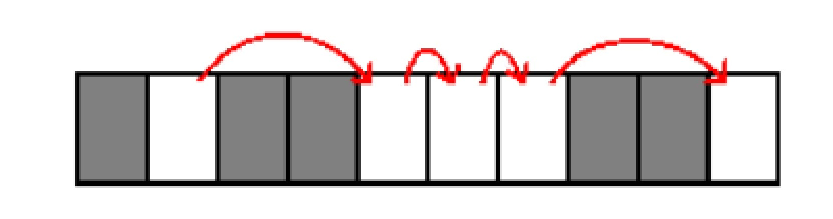
\includegraphics[width=1.5in]{fig1}
%\caption{Basic Linked List}\label{fig_1}
%\end{figure}
%
%\textbf{Sequential fit} is a set of similar allocation strategies including first fit, next fit and best fit. They all use no more than a double linked list to manage the free chunks. When a memory request comes, first fit starts searching the list from the beginning and stops at the first time it meets a free chunk that fulfills the request. It splits the free chunk into two pieces, one of which is in the request size and returned to the application whilst the remainder is inserted back to the list. One big disadvantage of first fit is poor locality, which increases the possibility of cache miss, thus increases the reference time as well as the total running time. Next fit also searches the free list one by one, but starting from where it finds the free chunk for the previous request. The first and next fit both continuously split large free chunks to smaller ones, which cannot be used for later large request, so they both suffer from big fragmentation. The best fit, on the other hand, goes through the whole free list before it makes a decision. So it guarantees to return the smallest free chunk in the list that meets the request, sometimes even the exact fit, hence it performs better in terms of fragmentation than first fit and next fit\cite{Johnstone:1998:MFP:301589.286864}. However, because it goes through the whole list every time there is a request, it costs a lot of time for allocation especially when the free list is very long.
%
%\begin{figure}[htbp]
%\centering
%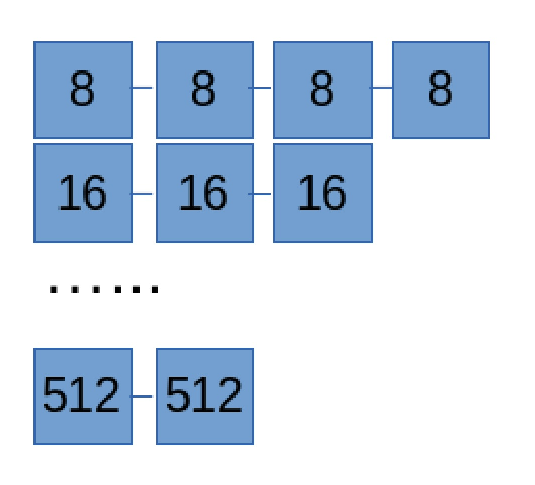
\includegraphics[width=1in]{fig2}
%\caption{Segregated free lists}\label{fig_2}
%\end{figure}
%\textbf{Segregated fit} keeps multiple free lists at the same time (Figure \ref{fig_2}) instead of managing one free list like what sequential fit does. Each of the free lists kept by segregated fit policy contains free chunks in the exact same size which is always a multiple of 8 bytes or a size in power of 2. This has also been known to increase the internal fragmentation (see section \ref{sec_fragmentation}). Each time there is a request of size \emph{n}, it only needs to fetch a free chunk from one of the free lists that corresponds to size \emph{n}. So it saves the allocation time by diminishing the searching time for a best fit whilst keeping a low fragmentation. But it harms a little of the deallocation time since it has to find the exact free list in the deallocated size before the freed chunk can be inserted to that list. What's more, it is possible that there is no available free chunk in the free list that corresponds to the request size, in which case the allocator will get a larger chunk from the next non-empty free list and split the chunk to meet the request. A variant of segregated fit differs only on returning a free chunk without aplitting it even if the chunk is much bigger than the request size. In this allocation strategy, the memory consumption is much higher because each chunk is in a fixed size and may be serving a much smaller request so that the extra size in that chunk can not be reused by other requests. But there is no denying this simplified segregated fit strategy is fast. This also shows there is clearly a trade-off between allocation time and memory consumption.
%
%\textbf{Coalescing} is a strategy which can be combined with or applied to the above allocation strategies, so can the ones introduced later. In order to save memory, most of the policies above choose to split a chunk before returning it to the application. This leads to more and more small chunks that cannot be used for big request. But some of these small chunks could be contiguous in the address space so that they can be concatenated to serve large request, in order to save memory. Coalescing policies try to concatenate contiguous free chunks into a bigger one, but when to apply coalescing remains adjustable in different allocators. This is because if an application request a chunk with size of \emph{n} right after it frees a chunk in the same size, the allocator may have coalesced the freed chunk but split it out from the concatenated chunk again to serve the same-size-request, which is a waste of computation. So instead of coalescing every time the application frees a chunk, some allocators apply coalescing in a fix frequency or once there is no big enough chunk that meets the request. In summary, whether the coalescing policy improves or diminishes the performance of an allocator really depends on the allocator itself and the allocation pattern of the application.
%
%\textbf{Searching strategy} refers to how an allocator manages and searches the free list(s). Some allocators keep the free list(s) in ascending or descending order in terms of address or size. It is quick for searching but may cause poor locality. Good locality refers to trying to allocate chunks that may be accessed subsequently in the application, on the same physical page, in order to minimize the cache misses in the operating system as a means of saving execution time. Searching strategy is quite influential to locality since it determines where subsequent requests should be located. On the other hand, when a chunk is freed and returned to the allocator, there are several ways to place it back in the free list(s), two of which are first-in-first-out (FIFO) and last-in-first-out (LIFO). FIFO strategy gives the most recently released chunk the least priority and places it at the end of the searching queue, whilst LIFO gives the most recently released chunk the highest priority so that it is more likely to be reused in a short time. There is no telling which one is better since it depends on other allocation strategies and the application itself.
%
%\textbf{Bitmap} is another combinable strategy that uses boolean flags to keep the status of chunks or free lists. When it stores the status of chunks, one bit usually represents whether a chunk is in use, and when it keeps the status of free lists, it usually means whether a free list is empty. The bitmap is designed to help the allocator to find an available chunk easily. It narrows the range down by searching the bitmap before searching a free chunk that meets the request.
%
%\textbf{Buddy system} is a well known algorithm which involves a special splitting mechanism. It always allocates memory in several fixed sizes and whenever it needs to split a chunk into two, it splits it in a fixed ratio repeatedly until it meets the smallest chunk that bigger than the request size. In this special splitting mechanism coalescing is fast because finding the other ``buddy'' generated from the same splitting is no more than a couple of simple mathematical computation. Even though the splitting ratio is adjustable, buddy systems still suffer from huge internal fragmentation.
%
%\subsection{Internal and External Fragmentation}
%\label{sec_fragmentation}
%Most of the memory allocators keep all the chunks in the size of multiple of 8 bytes due to the operating system requirements. In these cases, all the memory requests from applications are rounded up to an alignment of 8 bytes before they are really allocated. So the returned chunk is always equal to or slightly bigger than the request size without the applications being aware of it. Then the little extra padding memory is neglected and cannot be used by the applications. This is always refered to as internal fragmentation. On the other hand, at any point of a running application, the memory allocator always hold some free chunks instead of returning them to the operating system, so that it can quickly respond to some memory request from the application using these free chunks. And some of these free chunks may be too small to serve bigger request and for some reason they cannot be coalesced neither (e.g., not next to any other free chunks). The number of these small chunks may increase when the application proceeds, which causes the application occupying more memory than it really needs. This is also known as external fragmentation. 
%
%Allocators always introduce fragmentation, in different degrees. Despite many attempts to minimize memory fragmentation in an efficient way, there is clearly a trade-off between running time and memory fragmentation. For instance allocators with coalescing policies reuse small free chunks by concatenating them whilst introducing more computation for coalescing. And both segregated fit and buddy systems suffer from high fragmentation but they always contribute to fast allocators. 
%
%\subsection{\emph{Dlmalloc}}
%\label{sec_dlmalloc}
%\emph{Dlmalloc} keeps two set of segregated lists for small and large size requests respectively. 
%\begin{figure}[htbp]
%\centering
%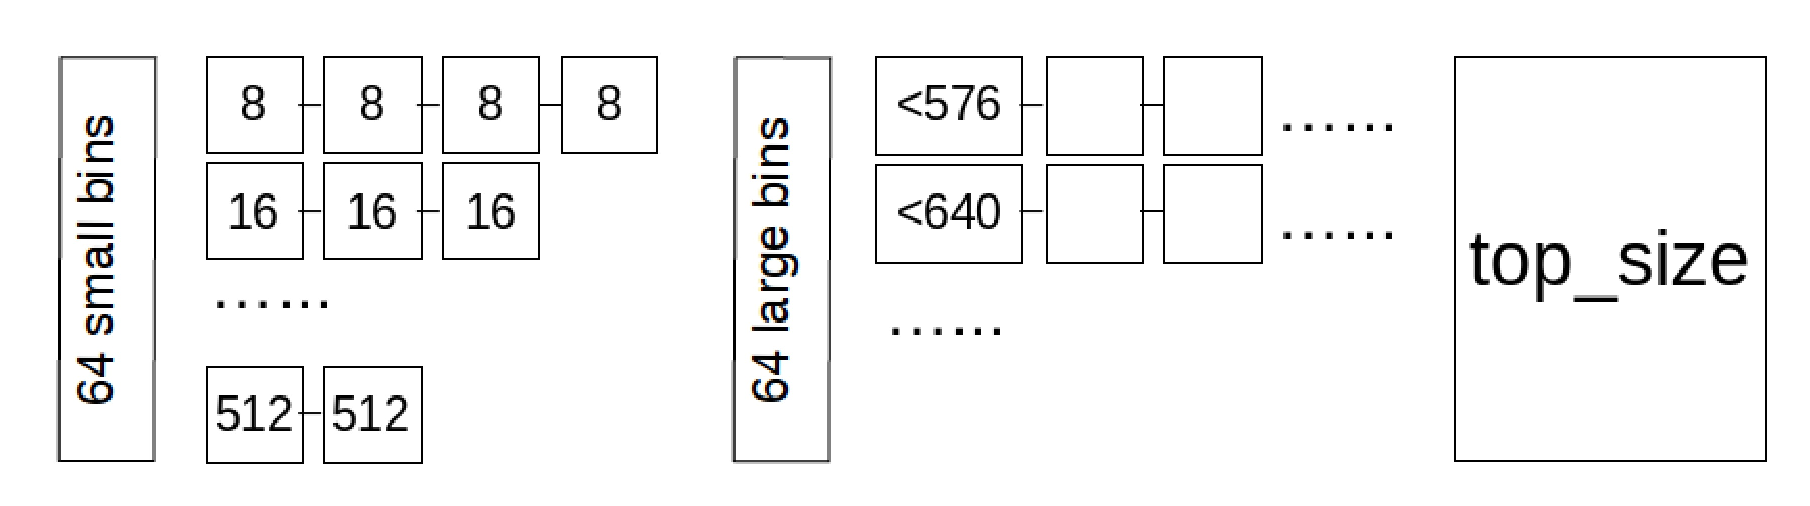
\includegraphics[width=0.4\textwidth]{fig7}
%\caption{structure of \emph{dlmalloc}}\label{fig_7}
%\end{figure}
%Each of the segregated lists is called a bin and there are 64 small bins and 64 large bins in \emph{dlmalloc} (Figure \ref{fig_7}). For small bins, each one contains chunks in the same size aligned to multiple of 8 bytes, which makes the largest chunk in small bins 512 bytes. Since chunks in the same small bin are in the exact same size, there is no need to sort the list, and insertion to or deletion from the list is very quick. For large bins, each bin is associated with a range of size which doesn't overlap with that of other bins. All the chunks larger than 512 bytes are stored in one of the large bins according to its size and kept in ascending order. So finding a chunk with a desired size requires a thorough search of an associated bin in the worst case. Apart from these segregated lists, \emph{dlmalloc} also keeps a top chunk, which is always at the end of the heap so that it can be extended or shrinked without affecting the data structure of other bins. The top chunk is used only when there is no available chunk in any bins that meets the memory request.
%
%\begin{figure}[htbp]
%\centering
%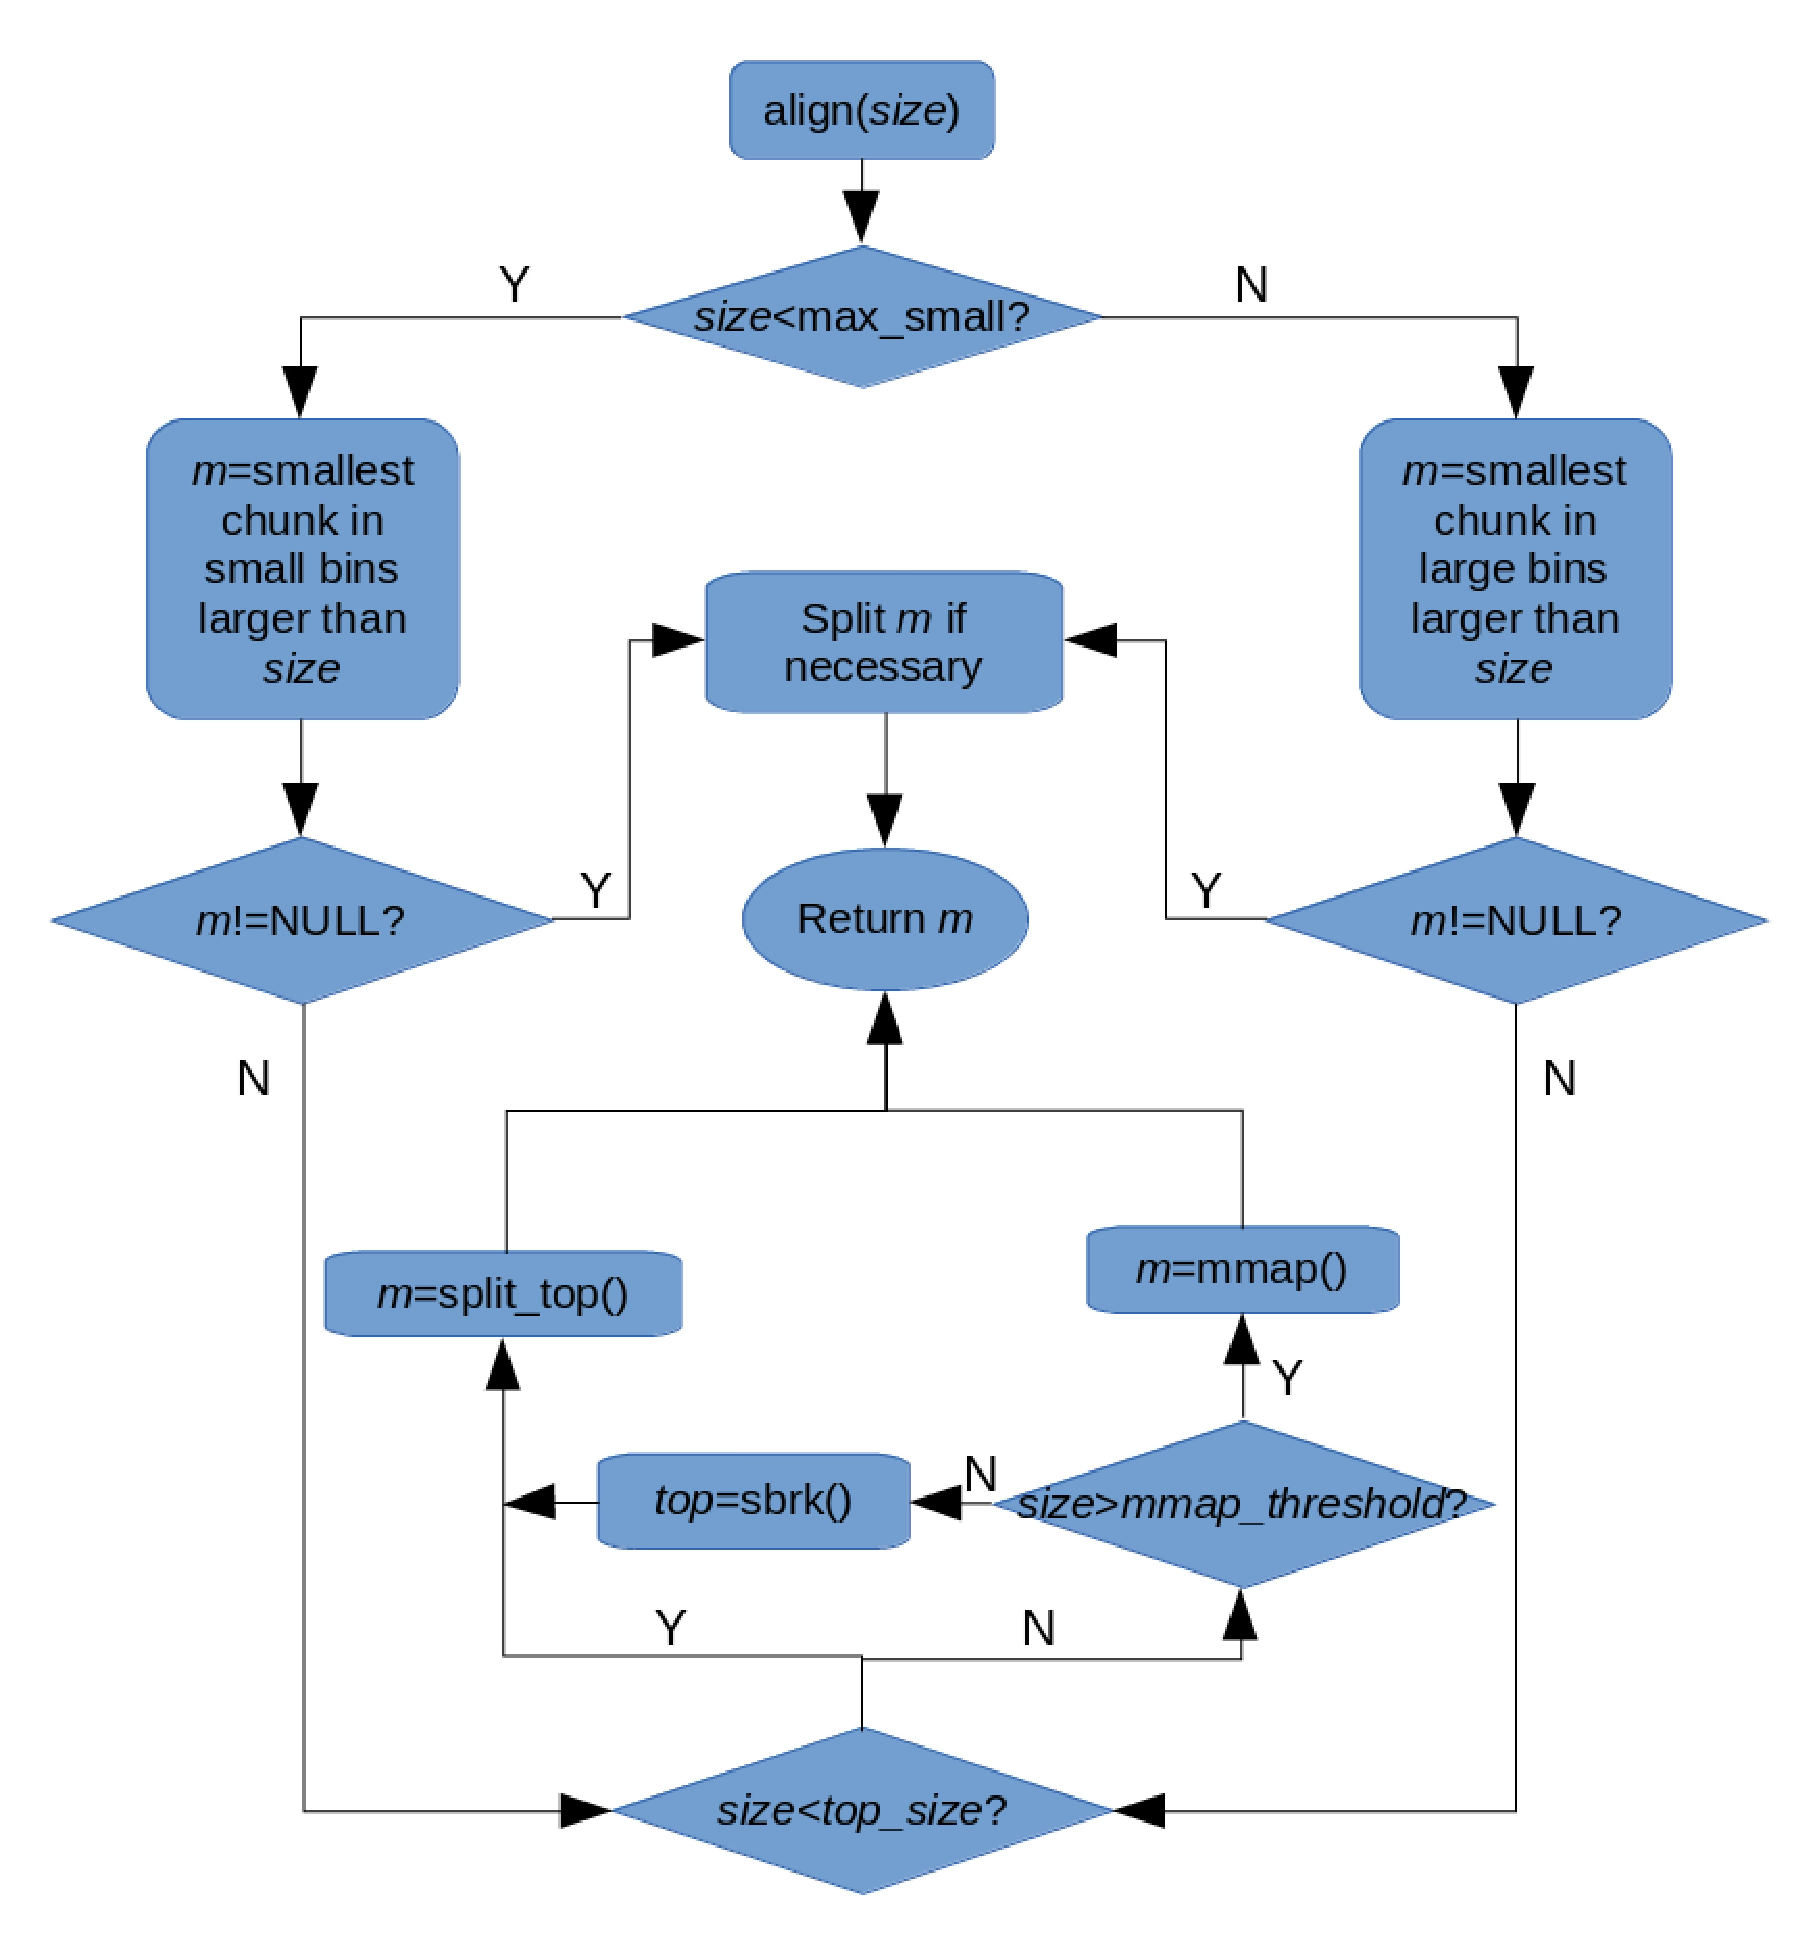
\includegraphics[width=0.4\textwidth]{fig8}
%\caption{allocation process of \emph{dlmalloc}}\label{fig_8}
%\end{figure}
%When a memory request from the application comes, \emph{dlmalloc} first rounds it up to a multiple of 8 bytes, then determine whether it belongs to small or large bins(Figure \ref{fig_8}). Either way, it searches the corresponding bin(s) based on the request size. If an available chunk that meets the requirement is found, it is returned to the application before which split may be applied if necessary. Otherwise, \emph{dlmalloc} tries to use the top chunk to serve the request by splitting the top chunk if the request size is smaller than the size of the top chunk, in which case the remainder is preserved as the new top chunk. If the request size is too large to be gotten from the top chunk, \emph{dlmalloc} uses an \emph{mmap}-like system call to allocate this size of memory from the operating system directly only when the request size is bigger than a pre-defined threshold. Otherwise it tries to extend the top chunk using \emph{sbrk}-like system call, so that the extended top chunk is big enough to cover the request.
%When a chunk is freed by the application, it is put back to one of the bins according to its size, after which \emph{dlmalloc} occasionally coalesces contiguous free chunks to create bigger chunks. If the top chunk is enlarged by combining free chunks next to it, it is also checked whether it is too large for the need of the application, in which case the top chunk may be shrinked. If the freed chunk was mapped directly from the system, it is released to system immediately. 
%There are several other details and techniques in \emph{dlmalloc} that are less relevant to our work, so we don't list them in this article. But they can be easily found in \emph{dlmalloc}'s source code.
